I tipi base fanno da atomi per le strutture di dati in un programma Go.
I tipi \textit{compositi} sono quindi le molecole create combinando i tipi di base in vari modi.
Ne esistono di quattro tipi: array, slice, map e struct.

Gli array e le struct sono tipi \textit{aggregati};
i loro valori sono concatenazioni di altri valori in memoria.
Gli array sono omogenei (i loro elementi hanno tutti lo stesso tipo) mentre le struct sono eterogenee.
Entrambi gli array e le struct sono di dimensioni fisse.
Al contrario, le slice e le map sono strutture di dati dinamici che crescono con l'aggiunta di valori.


\section{Gli array}
\label{sec:gli_array}
%
Un array è una sequenza a lunghezza fissa di zero o più elementi di un particolare tipo.
A causa della loro lunghezza fissa, gli array sono raramente utilizzati in modo diretto in Go.
Le slice, che possono crescere e ridursi, sono molto più versatili, ma per capire le slice bisogna prima capire le matrici.

I singoli elementi dell'array sono accessibili con la notazione indice convenzionale, dove gli indici vanno da zero a uno in meno rispetto alla lunghezza dell'array.
La funzione integrata \verb|len| restituisce il numero di elementi nell'array.
\begin{lstlisting}[frame=single, label={lst:lstlisting3-1.1}]
var a [3]int             // array di 3 interi
fmt.Println(a[0])        // stampa il primo elemento
fmt.Println(a[len(a)-1]) // stampa l'ultimo elemento

// Stampa gli indici e gli elementi.
for i, v := range a {
    fmt.Printf(%*``*\)%d %d\n%*''*\), i, v)
}

// Stampa solo gli elementi.
for _, v := range a {
    fmt.Printf(%*``*\)%d\n%*''*\), v)
}
\end{lstlisting}
Per impostazione predefinita, gli elementi di una nuova variabile di matrice sono inizialmente impostati al valore zero per il particolare tipo di elemento, che è \verb|0| per i numeri.
Possiamo usare un \textit{array letterale} per inizializzare un array con una lista di valori:
\begin{lstlisting}[frame=single, label={lst:lstlisting3-1.2}]
var q [3]int = [3]int{1, 2, 3}
var r [3]int = [3]int{1, 2}
fmt.Println(r[2])
\end{lstlisting}
Output:
\begin{lstlisting}[language=bash, frame=L, label={lst:lstlisting3-1.3}]
0
\end{lstlisting}
In un array letterale, se un ellissi ``\verb|...|'' appare al posto della lunghezza, la lunghezza dell'array è determinata dal numero di inizializzatori.
La definizione di \verb|q| può essere semplificata a:
\begin{lstlisting}[frame=single, label={lst:lstlisting3-1.4}]
q := [...]int{1, 2, 3}
fmt.Println(%*``*\)%T\n%*''*\), q)
\end{lstlisting}
Output:
\begin{lstlisting}[language=bash, frame=L, label={lst:lstlisting3-1.5}]
[3]int
\end{lstlisting}
La dimensione di un array fa parte del suo tipo, quindi \verb|[3]int| e \verb|[4]int| sono tipi diversi.
La dimensione deve essere un'espressione costante, cioè un'espressione il cui valore può essere calcolato mentre il programma viene compilato.
\begin{lstlisting}[frame=single, label={lst:lstlisting3-1.6}]
q := [3]int{1, 2, 3}
q = [4]int{1, 2, 3, 4} // compile error: impossibile assegnare
                       // [4]int a [3]int
\end{lstlisting}
La sintassi letterale è simile per array, slice, map e struct.
La forma specificata sopra è una lista ordinata di valori, ma è anche possibile specificare una lista di coppie di indici e valori, come:
\begin{lstlisting}[frame=single, label={lst:lstlisting3-1.7}]
type Currency int

const (
    USD Currency = iota
    EUR
    GBP
)

symbol := [...]string{USD: %*``\dollar''*\), EUR: %*``€''*\), GBP: %*``£''*\)}

fmt.Println(GBP, symbol[GBP])
\end{lstlisting}
Output:
\begin{lstlisting}[language=bash, frame=L, label={lst:lstlisting3-1.8}]
2 %*£*\)
\end{lstlisting}
Se il tipo di elemento di un array è comparabile, anche il tipo di array è comparabile, quindi possiamo confrontare direttamente due array di quel tipo usando l'operatore \verb|==|, che riporta se tutti gli elementi corrispondenti sono uguali.
L'operatore \verb|!=| è la sua negazione.

Come esempio, la funzione \verb|Sum256| nel pacchetto \verb|crypto/sha256| produce l'hash crittografico SHA256 o il \textit{digest} di un messaggio memorizzato in una slice di byte arbitraria.
Il digest ha 256 bit, quindi il suo tipo è \verb|[32]byte|.
Se due digest sono uguali, è estremamente probabile che i due messaggi siano uguali;
se i digest differiscono, i due messaggi sono diversi.
Questo programma stampa e confronta i digest SHA256 di ``\verb|x|'' e ``\verb|X|'':
\begin{lstlisting}[frame=single, label={lst:lstlisting3-1.9}]
import %*``*\)crypto/sha256%*''*\)

func main() {
    c1 := sha256.Sum256([]byte(%*``*\)x%*''*\)))
    c2 := sha256.Sum256([]byte(%*``*\)X%*''*\)))
    fmt.Printf(%*``*\)%x\n%x\n%t\n%T\n%*''*\), c1, c2, c1 == c2, c1)
}
\end{lstlisting}
Output:
\begin{lstlisting}[language=bash, frame=L, label={lst:lstlisting3-1.10}]
2d711642b726b04401627ca9fbac32f5c8530fb1903cc4db02258717921a4881
4b68ab3847feda7d6c62c1fbcbeebfa35eab7351ed5e78f4ddadea5df64b8015
false
[32]uint8
\end{lstlisting}
I due ingressi differiscono di un solo bit, ma molti bit dei loro digest sono diversi fra loro.

Quando viene chiamata una funzione, una copia di ogni valore di argomento viene assegnata alla variabile parametro corrispondente, quindi la funzione riceve una copia, non l'originale.
Il passaggio di array di grandi dimensioni in questo modo può essere inefficiente, e qualsiasi modifica apportata dalla funzione agli elementi di array influisce solo sulla copia, non sull'originale.
A questo proposito, Go tratta gli array come qualsiasi altro tipo, ma questo comportamento è diverso dai linguaggi che implicitamente passano gli array \textit{per riferimento}.

Naturalmente, possiamo passare esplicitamente un puntatore ad un array in modo che tutte le modifiche che la funzione apporta agli elementi array siano visibili al chiamante.
Questa funzione azzera il contenuto di un array \verb|[32]byte|:
\begin{lstlisting}[frame=single, label={lst:lstlisting3-1.11}]
func zero(ptr *[32]byte) {
    *ptr = [32]byte{}
}
\end{lstlisting}
L'array letterale \verb|[32]byte{}| produce un array di 32 byte.
Ogni elemento dell'array ha il valore zero per del byte, ovvero la traduzione di \verb|0| in byte.

L'utilizzo di un puntatore a un array è efficiente e consente alla funzione chiamata di mutare la variabile del chiamante, ma gli array sono ancora intrinsecamente inflessibili a causa delle loro dimensioni fisse.
La funzione \verb|zero| non accetta un puntatore a una variabile di \verb|[16]byte|, per esempio, né c'è alcun modo di aggiungere o rimuovere elementi di matrice.
Per queste ragioni, oltre a casi speciali come l'hash di dimensione fissa di SHA256, gli array sono raramente usati come parametri di funzione o come risultati;
invece, usiamo le slice.

\section{Le slice}
\label{sec:le_slice}
%
Le slice rappresentano sequenze di lunghezza variabile di elementi, tutti dello stesso tipo.
Un tipo slice è scritto \verb|[]T|, dove gli elementi sono di tipo \verb|T|: assomiglia ad un array senza una dimensione.

Le matrici e le slice sono intimamente connesse.
Una slice è una struttura dati leggera che dà accesso a una sottosequenza (o anche a tutti) degli elementi di un array, che è noto come \textit{array sottostante} della slice.
Una slice ha tre componenti: un puntatore, una lunghezza e una capacità.
Il puntatore punta al primo elemento dell'array che è raggiungibile attraverso la slice (non necessariamente il primo elemento dell'array).
La lunghezza è il numero di elementi della slice, per cui non può superare la capacità della stessa;
la capacità è di solito il numero di elementi tra l'inizio della slice e la fine dell'array sottostante.
Le funzioni built-in \verb|len| e \verb|cap| restituiscono tali valori.

Più slice possono condividere lo stesso array sottostante e possono riferirsi a parti sovrapposte di esso.
La figura mostra un array di stringhe per i mesi dell'anno e due slice sovrapposte di esso.
L'array è dichiarato come:
\begin{lstlisting}[label={lst:lstlisting3-2.1}]
months := [...]string{1: %*``*\)January%*''*\), /* ... */, 12: %*``*\)December%*''*\)}
\end{lstlisting}
quindi gennaio è \verb|months[1]| e dicembre è \verb|months[12]|.
Si è lasciato fuori dalla dichiarazione l'indice \verb|0| così da inizializzare l'elemento ad esso relativo ad una stringa vuota.

L'\textit{operatore di slice} \verb|s[i:j]|, dove \verb|0|$\le$\verb|i|$\le$\verb|j|$\le$\verb|cap(s)|, crea una nuova slice che si riferisce agli elementi dalla posizione \verb|i| fino alla posizione \verb|j-1| della sequenza \verb|s|, dove \verb|s| può essere una variabile array, un puntatore ad un array o un'altra slice.
La slice risultante ha \verb|j-i| elementi.
Se \verb|i| viene omesso, è come aver inserito \verb|0|, analogamente se \verb|j| viene omesso, è come aver inserito \verb|len(s)|.
Così la slice \verb|months[1:13]| si riferisce all'intera gamma dei mesi validi, così come la slice \verb|months[1:]|;
mentre la slice \verb|months[:]| si riferisce all'intero array (dall'elemento \verb|0| all'elemento \verb|12|).

Un esempio di slice sulla sequenza \verb|months|:
\begin{center}
    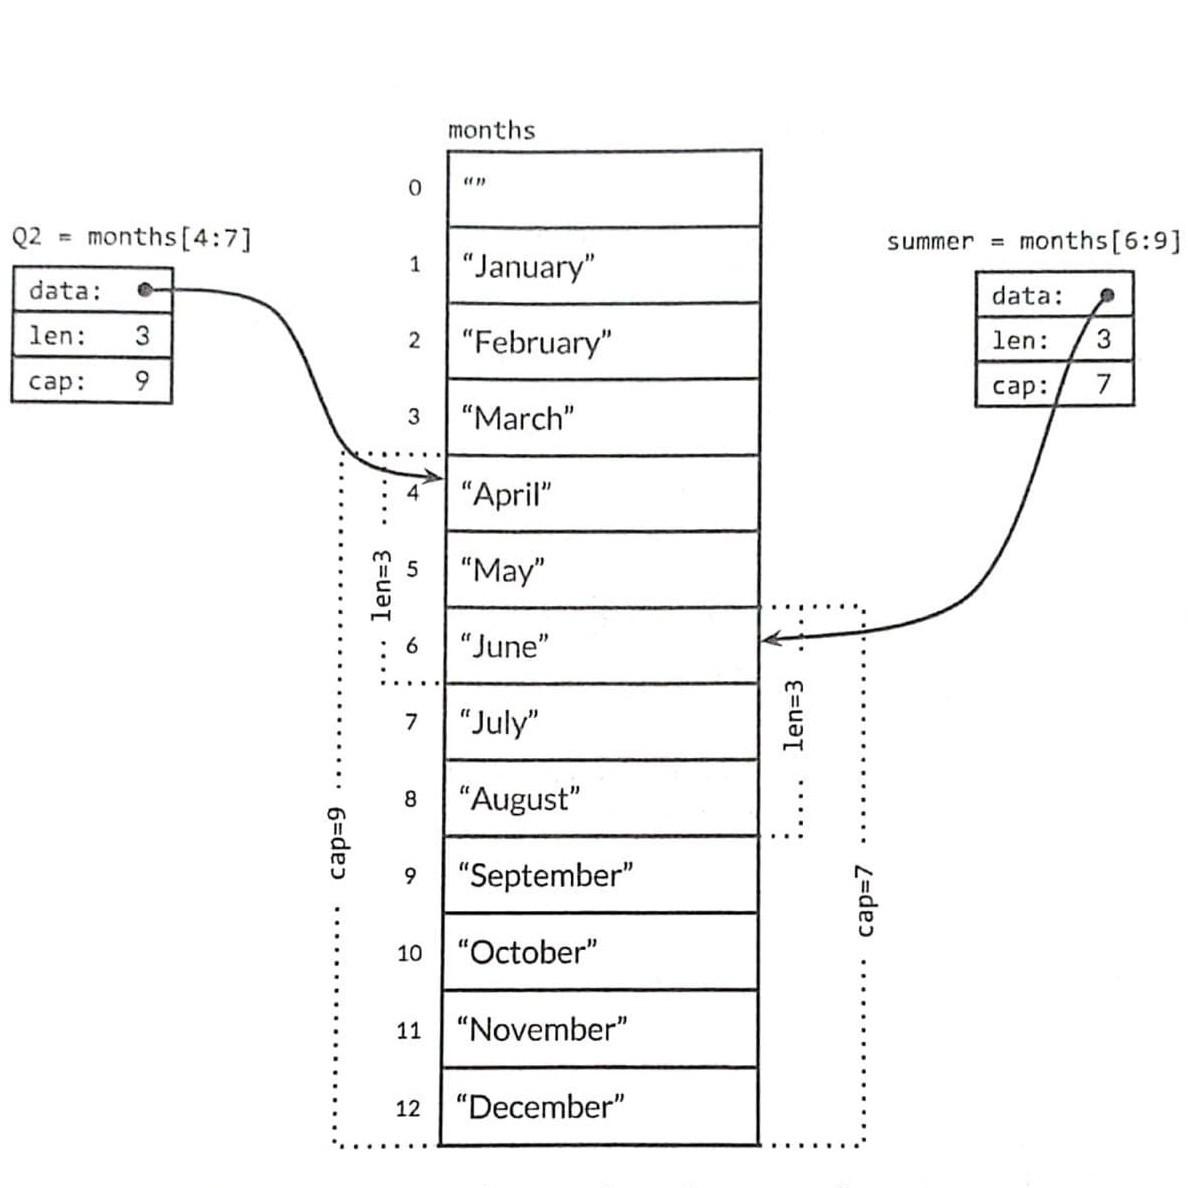
\includegraphics[width=0.5\linewidth]{figures/figura3.1}
\end{center}
\begin{lstlisting}[frame=single, label={lst:lstlisting3-2.2}]
Q2 := months[4:7]
summer := months[6:9]
fmt.Println(Q2)
fmt.Println(summer)
\end{lstlisting}
Output:
\begin{lstlisting}[language=bash, frame=L, label={lst:lstlisting3-2.3}]
[%*``*\)April%*''*\) %*``*\)May%*''*\) %*``*\)June%*''*\)]
[%*``*\)June%*''*\) %*``*\)July%*''*\) %*``*\)August%*''*\)]
\end{lstlisting}
Nell'espressione delle slice, andare oltre \verb|cap(s)| si ottiene una situazione di \verb|panic|, ma andare oltre \verb|len(s)| si ottiene l'estensione della slice, quindi il risultato può diventare più ricco di quello di partenza.
\begin{lstlisting}[frame=single, label={lst:lstlisting3-2.4}]
fmt.Println(summer[:20])    // panic: fuori portata

endlessSummer := summer[:5] // estende una slice entro la sua
                            // capacit%*\textit{à}*\)
fmt.Println(endlessSummer)
\end{lstlisting}
Output:
\begin{lstlisting}[language=bash, frame=L, label={lst:lstlisting3-2.5}]
[June July August September October]
\end{lstlisting}
Poiché una slice contiene un puntatore ad un elemento di un array, passare una slice ad una funzione permette alla funzione di modificare gli elementi dell'array sottostante.
In altre parole, copiare una slice vuol dire creare un \textit{alias} per l'array sottostante.

Uno \textit{slice literal} si presenta come un array literal, una sequenza di valori separati da virgole racchiusi in parentesi graffe, con la dimensione non data.
Questo crea implicitamente una variabile array della giusta dimensione e produce una slice che punta ad essa.
Come con gli array literal, gli slice literal possono specificare in ordine i valori, o assegnare esplicitamente loro gli indici, oppure usare un mix dei due stili.

A differenza degli array, le slice non sono confrontabili, quindi non possiamo usare l'operatore \verb|==| per verificare se due slice contengono gli stessi elementi.
Per i tipi di riferimento come puntatori e channel, l'operatore \verb|==| verifica la \textit{reference identity}, cioè se le due entità riferiscono alla stessa cosa.
La scelta più sicura è quella di non permettere in alcun caso il confronto fra slice.

L'unico confronto legale è con \verb|nil|:
\begin{lstlisting}[frame=single, label={lst:lstlisting3-2.6}]
if summer == nil { /* ... */ }
\end{lstlisting}
Il valore zero di un tipo di slice è \verb|nil|.
Una slice nil non ha un array sottostante.
La slice nil ha lunghezza e capacità zero, ma ci sono anche le slice non nil di lunghezza e capacità zero, come \verb|[]int{}|.
Il valore nil di un particolare tipo di slice può essere scritto usando un'espressione di conversione come \verb|[]int(nil)|.

A meno che non sia chiaramente documentato il contrario, le funzioni Go trattano tutte le slice di lunghezza zero allo stesso modo, sia nil che non nil.

La funzione incorporata \verb|make| crea una slice di un tipo di elemento specificato, e di una certa lunghezza e capacità.
L'argomento capacità può essere omesso, nel qual caso si intende uguale alla lunghezza.
\begin{lstlisting}[frame=single, label={lst:lstlisting3-2.7}]
make([]T, len)
make([]T, len, cap) // uguale a make([]T, cap)[:len]
\end{lstlisting}
La funzione \verb|make| crea una variabile array senza nome e ne restituisce una slice;
l'array è accessibile solo attraverso la slice restituita.
Nella prima forma, la slice è una vista dell'intero array.
Nel secondo, la slice è una vista solo dei primi \verb|len| elementi dell'array, ma la sua capacità include l'intero array.
Gli elementi aggiuntivi sono quindi accantonati per una crescita futura della slice.

La funzione built-in \verb|append| aggiunge elementi alle slice.

Di solito non sappiamo se una determinata chiamata ad \verb|append| causerà una riallocazione, quindi non possiamo supporre che la slice originale punti allo stesso array della slice risultante, né che si riferisca a una diversa.
Allo stesso modo, non dobbiamo presumere che le assegnazioni ad elementi della vecchia slice si rifletteranno (o non si rifletteranno) sulla nuova slice.
Di conseguenza, è normale assegnare il risultato di una chiamata ad \verb|append| alla stessa variabile slice il cui valore è stato passato alla chiamata della funzione \verb|append|:
\begin{lstlisting}[frame=single, label={lst:lstlisting3-2.8}]
var runes []rune
for _, r := range %*``*\)Hello, World%*''*\) {
    runes = append(runes, r)
}
fmt.Printf(%*``*\)%q\n%*''*\), runes)
\end{lstlisting}
Output:
\begin{lstlisting}[language=bash, frame=L, label={lst:lstlisting3-2.9}]
[`H' `e' `l' `l' `o' `,' `W' `o' `r' `l' `d']
\end{lstlisting}
\
Inoltre, la funzione \verb|append| ci permette di aggiungere più di un nuovo elemento, o anche una slice intera dello stesso tipo.
\begin{lstlisting}[frame=single, label={lst:lstlisting3-2.10}]
var x []int
x = append(x, 1)
x = append(x, 2, 3)
x = append(x, 4, 5, 6)
x = append(x, x...) // Aggiunge la slice x
fmt.Println(x)
\end{lstlisting}
Output:
\begin{lstlisting}[language=bash, frame=L, label={lst:lstlisting3-2.11}]
[1 2 3 4 5 6 1 2 3 4 5 6]
\end{lstlisting}
Verrà spiegato più in avanti il perché dell'ellissi ``\verb|...|'' nella chiamata alla funzione \verb|append| nell'ultimo esempio.

Una slice può essere usata per implementare uno stack.
Data uno stack di slice inizialmente vuota, possiamo spingere un nuovo valore alla fine della slice con \verb|append|:
\begin{lstlisting}[frame=single, label={lst:lstlisting3-2.12}]
stack = append(stack, v) // push v
\end{lstlisting}
La testa dello stack è l'ultimo elemento:
\begin{lstlisting}[frame=single, label={lst:lstlisting3-2.13}]
top := stack[len(stack)-1] // top dello stack
\end{lstlisting}
e la restrizione dello stack effettuando il pop dell'elemento:
\begin{lstlisting}[frame=single, label={lst:lstlisting3-2.14}]
stack := stack[:len(stack)-1] // pop
\end{lstlisting}
Per rimuovere un elemento dal centro di una slice, conservando l'ordine degli elementi rimanenti, si usa \verb|copy| per far scorrere gli elementi con il numero più alto verso il basso di uno a riempire lo spazio vuoto generato:
\begin{lstlisting}[frame=single, label={lst:lstlisting3-2.15}]
func remove(slice []int, i int) []int {
    copy(slice[i:], slice[i+1:])
    return slice[:len(slice)-1]
}

func main() {
    s := []int{5, 6, 7, 8, 9}
    fmt.Println(remove(s, 2))
}
\end{lstlisting}
Output:
\begin{lstlisting}[language=bash, frame=L, label={lst:lstlisting3-2.16}]
[5 6 8 9]
\end{lstlisting}

\section{Maps}
\label{sec:maps}
%
La tabella hash è una delle più ingegnose e versatili di tutte le strutture dati.
Si tratta di una raccolta non ordinata di coppie chiave/valore in cui tutte le chiavi sono distinte e il valore associato a una determinata chiave può essere recuperato, aggiornato o rimosso utilizzando in media un numero costante di confronti di chiave, non importa quanto grande sia la tabella hash.

In Go, una \textit{map} è un riferimento a una tabella hash, ed è scritto \verb|map[K]V|, dove \verb|K| e \verb|V| sono i tipi delle sue chiavi e dei suoi valori.
Tutte le chiavi in una determinata map sono dello stesso tipo e tutti i valori sono dello stesso tipo, ma le chiavi non devono necessariamente essere dello stesso tipo dei valori.
Il tipo di chiave \verb|K| deve essere comparabile usando \verb|==|, in modo che la map possa verificare se una determinata chiave è uguale a una già all'interno di essa.
Non ci sono restrizioni sul tipo di valore \verb|V|.

La funzione integrata \verb|make| può essere utilizzata per creare una map:
\begin{lstlisting}[label={lst:lstlisting3-3.1}]
ages := make(map[string]int) // map da string a int
\end{lstlisting}
Possiamo anche usare una \textit{map literal} per creare una nuova map popolata da alcune coppie chiave/valore iniziali:
\begin{lstlisting}[frame=single, label={lst:lstlisting3-3.2}]
ages := map[string]int {
    %*``*\)alice%*''*\):   31,
    %*``*\)charlie%*''*\): 34,
}
\end{lstlisting}
Ciò equivale a
\begin{lstlisting}[frame=single, label={lst:lstlisting3-3.3}]
ages := make(map[string]int)
ages[%*``*\)alice%*''*\)] = 31
ages[%*``*\)charlie%*''*\)] = 34
\end{lstlisting}
quindi un'espressione alternativa per una nuova map vuota è \verb|map[string]int{}|.

Gli elementi della map sono accessibili attraverso la consueta notazione:
\begin{lstlisting}[frame=single, label={lst:lstlisting3-3.4}]
ages[%*``*\)alice%*''*\)] = 32
fmt.Println(ages[%*``*\)alice%*''*\)])
\end{lstlisting}
Output:
\begin{lstlisting}[language=bash, frame=L, label={lst:lstlisting3-3.5}]
32
\end{lstlisting}
e rimosso con la funzione integrata \verb|delete|:
\begin{lstlisting}[language=go, frame=single, label={lst:lstlisting3-3.6}]
delete(ages, %*``*\)alice%*''*\)) // rimuovere elemento et%*\textit{à}*\)[%*``*\)alice%*''*\)]
\end{lstlisting}
Tutte le operazioni sono sicure anche se l'elemento non è nella map;
una ricerca di una chiave che non è presente nella map restituisce il valore zero per il suo tipo, così, per esempio, il seguente codice funziona anche quando ``bob'' non è ancora una chiave della map perché il valore di \verb|ages["bob"]| sarà \verb|0|.
\begin{lstlisting}[frame=single, label={lst:lstlisting3-3.7}]
ages[%*``*\)bob%*''*\)]++
\end{lstlisting}
Ma un elemento della map non è una variabile, per cui non si può ottenere il suo indirizzo
\begin{lstlisting}[frame=single, label={lst:lstlisting3-3.8}]
_ = &ages[%*``*\)bob%*''*\)] // compile error: impossibile prendere
                // l'indirizzo di un elemento di map
\end{lstlisting}
Il valore zero per una map è \verb|nil|, cioè un riferimento a nessuna tabella hash.
\begin{lstlisting}[frame=single, label={lst:lstlisting3-3.9}]
var ages map[string]int
fmt.Println(ages == nil)
fmt.Println(len(ages) == 0)
\end{lstlisting}
Output:
\begin{lstlisting}[language=bash, frame=L, label={lst:lstlisting3-3.10}]
true
true
\end{lstlisting}
La maggior parte delle operazioni sulle map, inclusi i cicli di ricerca, \verb|delete|, \verb|len| e \verb|range|, sono sicure da eseguire su una map di riferimento nil, poiché si comporta come una mappa vuota.
Ma la memorizzazione di una map nil provoca panic:
\begin{lstlisting}[frame=single, label={lst:lstlisting3-3.11}]
ages[%*``*\)carol%*''*\)] = 21 // panic: assegnazione ad una map nil
\end{lstlisting}
È necessario allocare la map prima di poter memorizzare in esso coppie chiave/valore.
In particolare, se si vuole sapere se una chiave è presente nella map, allora si può effettuare una chiamata:
\begin{lstlisting}[frame=single, label={lst:lstlisting3-3.12}]
age, ok = ages[%*``*\)bob%*''*\)]
\end{lstlisting}
In cui il primo valore contiene il valore associato alla chiave \verb|bob| nella map (se presente), mentre il secondo contiene un valore booleano che indica se la chiave è presente o meno nella map.

Come nelle slice, le map non possono essere confrontate fra loro;
l'unico confronto legale è con \verb|nil|.

\section{Struct}
\label{sec:struct}
%
Una \textit{struct} è un tipo di dati aggregato che raggruppa insieme zero o più valori denominati di tipi arbitrari in una singola entità.
Ogni valore è detto \textit{campo}.

Queste due istruzioni dichiarano un tipo di struct chiamato \verb|Employee| e una variabile chiamata \verb|dilbert| che è un'istanza di un \verb|Employee|:
\begin{lstlisting}[frame=single, label={lst:lstlisting3-4.1}]
type Employee struct {
    ID 	      int
    Name      string
    Address   string
    DoB       time.Time
    Position  string
    Salary    int
    ManagerID int
}

var dilbert Employee
\end{lstlisting}
I singoli campi di \verb|dilbert| sono accessibili usando la notazione a punti (\verb|dilbert.Name| e \verb|dilbert.DoB|).
Poiché \verb|dilbert| è una variabile, anche i suoi campi sono variabili, quindi possiamo assegnare ad un campo:
\begin{lstlisting}[frame=single, label={lst:lstlisting3-4.2}]
dilbert.Salary -= 5000
\end{lstlisting}
o prendere il suo indirizzo e accedervi tramite un puntatore:
\begin{lstlisting}[frame=single, label={lst:lstlisting3-4.3}]
position := &dilbert.Position
*position = %*``*\)Senior %*''*\) + *position
\end{lstlisting}
La notazione a punti funziona anche con un puntatore a una struct:
\begin{lstlisting}[frame=single, label={lst:lstlisting3-4.4}]
var employeeOfTheMonth *Employee = &dilbert
employeeOfTheMonth.Position += %*``*\) (proactive team player)%*''*\)
\end{lstlisting}
Dove l'ultima istruzione è equivalente a
\begin{lstlisting}[frame=single, label={lst:lstlisting3-4.5}]
(*employeeOfTheMonth).Position += %*``*\) (proactive team player)%*''*\)
\end{lstlisting}
I campi sono di solito scritti uno per riga, con il nome del campo che precede il suo tipo, ma i campi consecutivi dello stesso tipo possono essere combinati, come con \verb|Name| e \verb|Address| qui:
\begin{lstlisting}[frame=single, label={lst:lstlisting3-4.6}]
type Employee struct {
    ID            int
    Name, Address string
    DoB           time.Time
    Position      string
    Salary        int
    ManagerID     int
}
\end{lstlisting}
Un tipo di struct denominato \verb|S| non può dichiarare un campo dello stesso tipo \verb|S|: un valore aggregato non può contenere se stesso.
Ma \verb|S| può dichiarare un campo del tipo di puntatore \verb|*S|, che ci permette di creare struct di dati ricorsive come liste concatenate e alberi.
Questo è illustrato nel codice qui sotto, che utilizza un albero binario per implementare un ordinamento di inserimento:
\begin{lstlisting}[frame=single, label={lst:lstlisting3-4.7}]
type tree struct {
    value       int
    left, right *tree
}

// Sorts ordina i valori in posizione.
func Sort(values []int) {
    var root *tree
    for _, v := range values {
        root = add(root, v)
    }
    appendValues(values[:0], root)
}

// appendValues aggiunge gli elementi di t ai valori
// in ordine e restituisce la slice risultante.
func appendValues(values []int, t *tree) []int {
    if t != nil {
        values = appendValues(values, t.left)
        values = append(values, t.value)
        values = appendValues(values, t.right)
    }
    return values
}

func add(t *tree, value int) *tree {
    if t == nil {
        // Equivalente a ritornare &tree{value:value}
        t = new(tree)
        t.value = value
        return t
    }
    if value < t.value {
        t.left = add(t.left, value)
    } else {
        t.right = add(t.right, value)
    }
    return t
}
\end{lstlisting}
Il valore zero per una struct è composto dai valori zero di ciascuno dei suoi campi.

Il tipo di struct senza campi è chiamato \textit{empty struct}, scritto \verb|struct{}|.

\subsection{Struct literal}
\label{subsec:struct_literal}%
Un valore di un tipo di struttura può essere scritto usando una \textit{struct literal} che specifica i valori per i suoi campi.
\begin{lstlisting}[frame=single, label={lst:lstlisting3-4-1.1}]
type Point struct { X, Y int }

p := Point{1, 2}
\end{lstlisting}
Ci sono due forme di struct literal.
La prima forma, mostrata sopra, richiede che sia specificato un valore per \textit{ogni} campo nell'ordine giusto.
Rende il codice fragile se l'insieme dei campi dovesse poi crescere o essere riordinato.
Di conseguenza, questa forma tende ad essere usata solo all'interno del pacchetto che definisce il tipo di struct, o con tipi di struct più piccoli per i quali esiste un'ovvia convenzione di ordinamento dei campi, come \verb|image.Point{x, y}| o \verb|color.RGBA{red, green, blue, alpha}|.

Più spesso, viene usata la seconda forma, in cui un valore di struct viene inizializzato elencando alcuni o tutti i nomi dei campi e i loro valori corrispondenti.
Se un campo è omesso in questo tipo di literal, viene impostato al valore zero per il suo tipo.

I valori di struct possono essere passati come argomenti alle funzioni e restituiti da esse.
Per esempio, questa funzione scala un ``Punto'' di un fattore specificato:
\begin{lstlisting}[frame=single, label={lst:lstlisting3-4-1.2}]
func Scale(p Point, factor int) Point {
    return Point{p.X * factor, p.Y * factor}
}

fmt.Println(Scale(Point{1, 2}, 5))
\end{lstlisting}
Output:
\begin{lstlisting}[language=bash, frame=L, label={lst:lstlisting3-4-1.3}]
{5 10}
\end{lstlisting}
Per efficienza, la struct più grande è solitamente passata a o restituita da funzioni indirettamente usando un puntatore
\begin{lstlisting}[frame=single, label={lst:lstlisting3-4-1.4}]
func Bonus(e *Employee, percent int) int {
    return e.Salary * percent / 100
}
\end{lstlisting}
e questo è necessario se la funzione deve modificare il suo argomento, poiché in un linguaggio call-by-value come Go, la funzione chiamata riceve solo una copia di un argomento, non un riferimento all'argomento originale.

\subsection{Confronto tra struct}
\label{subsec:confronto_tra_struct}%
Se tutti i campi di una struct sono comparabili, la struct stessa è comparabile, quindi due espressioni di quel tipo possono essere confrontate usando \verb|==| o \verb|!=|.
L'operazione \verb|==| confronta i campi corrispondenti delle due struct in ordine, quindi le due espressioni stampate qui sotto sono equivalenti:
\begin{lstlisting}[frame=single, label={lst:lstlisting3-4-2.1}]
type Point struct { X, Y int }

p := Point{1, 2}
q := Point{2, 1}
fmt.Println(p.X == q.X && p.Y == q.Y)
fmt.Println(p == q)
\end{lstlisting}
Output:
\begin{lstlisting}[language=bash, frame=L, label={lst:lstlisting3-4-2.2}]
false
false
\end{lstlisting}

\subsection{Struct embedding e campi anonimi}
\label{subsec:struct_embedding_e_campi_anonimi}%
Un insolito meccanismo \textit{struct embedding} ci permette di usare un tipo di struct detto \textit{campo anonimo} di un altro tipo di struct, fornendo una comoda scorciatoia sintattica in modo che una semplice espressione puntiforme come \verb|x.f| possa rappresentare una catena di campi come \verb|x.d.e.f|.
Dati le seguenti struct:
\begin{lstlisting}[frame=single, label={lst:lstlisting3-4-3.1}]
type Circle struct {
    X, Y, Radius int
}

type Wheel struct {
    X, Y, Radius, Spokes int
}
\end{lstlisting}
conviene raccogliere i campi uguali a individuare una nuova struct
\begin{lstlisting}[frame=single, label={lst:lstlisting3-4-3.2}]
type Point struct {
    X, Y int
}
type Circle struct {
    Center Point
    Radius int
}

type Wheel struct {
    Circle Circle
    Spokes int
}
\end{lstlisting}
L'applicazione diventerebbe più chiara, ma questo cambiamento renderebbe anche l'accesso ai campi di ``Wheel'' più prolisso:
\begin{lstlisting}[frame=single, label={lst:lstlisting3-4-3.3}]
var w Wheel
w.Circle.Center.X = 8
w.Circle.Center.Y = 8
w.Circle.Radius = 5
w.Spokes = 20
\end{lstlisting}
Go ci permette di dichiarare un campo con un tipo ma senza nome;
tali campi sono chiamati \textit{campi anonimi}.
Il tipo di campo deve essere un tipo con nome o un puntatore a un tipo con nome.
Sotto, \verb|Circle| e \verb|Wheel| hanno un campo anonimo ciascuno.
Diciamo che un \verb|Point| è \textit{incorporato} all'interno di \verb|Circle|, e un \verb|Circle| è incorporato all'interno di \verb|Wheel|.
\begin{lstlisting}[frame=single, label={lst:lstlisting3-4-3.4}]
type Circle struct {
    Point
    Radius int
}

type Wheel struct {
    Circle
    Spokes int
}
\end{lstlisting}
Grazie all'incorporazione, possiamo fare riferimento ai nomi alle foglie dell'albero implicito senza dare i nomi intermedi:
\begin{lstlisting}[frame=single,label={lst:lstlisting3-4-3.5}]
var w Wheel
w.X = 8	     // equivalente a w.Circle.Point.X = 8
w.Y = 8	     // equivalente a w.Circle.Point.Y = 8
w.Radius = 5 // equivalente a w.Circle.Radius = 5
w.Spokes = 20
\end{lstlisting}
Poiché i campi ``anonimi'' hanno nomi impliciti, non è possibile avere due campi anonimi dello stesso tipo perché in tal caso i loro nomi entrerebbero in conflitto.

Il tipo struct esterno guadagna non solo i campi del tipo embedded ma anche i suoi metodi.
Questo meccanismo è il modo principale in cui i comportamenti degli oggetti complessi sono composti da quelli più semplici.
La \textit{composizione} è centrale per la programmazione orientata agli oggetti in Go.

